\documentclass{article}
\usepackage[english]{babel}
\usepackage[utf8x]{inputenc}
\usepackage{amsmath}
\usepackage{amsfonts}
\usepackage{mathtools}
\usepackage{amssymb}
\usepackage{graphicx}
\usepackage{amsthm}
\usepackage[colorinlistoftodos]{todonotes}
\usepackage{mathtools}
\usepackage{graphicx}

\title{CTA200 assignemnt 3 Q3}
\author{Ruyi Xu }
\date{May 2022}

\begin{document}

\maketitle
\newpage
\section{Q1}
\subsection{Method}
The equation given, $c=x+iy, z_{i+1} = z_{i}+c$ is given is the Mandelbrot set, the iteration of the function $z_{i+1} = z_{i}+c$ is done using a for loop where divergence is determined by the value of the function at a certain iteration. we are given the bounds for $x$ and $y$ where $|x|,|y|\leq 2$. To plot the density of divergent and bounded points, Binary operators (true) and (false) are used to determine what color a point should be. here 2 forms of plots are given for fig 1, a color gradient is used to illustrate density of divergent points and fig 1 illustrates a Boolean true/false figure.\\
\subsection{Results}
The results of the equation gives a geometric shape developing along the imaginary and real axis where the region has denser points of divergence compared to the other points. Other than that from fig 1.2 we can also observe that along the regions of divergence is also symmetrical along the axis and that each smaller geometric shpe further from the origin is a repeat of the same shape but smaller in the negative real direction and in both imaginary directions.
\newpage
\begin{figure}
\subsection{Figures for Q1}
    \centering
    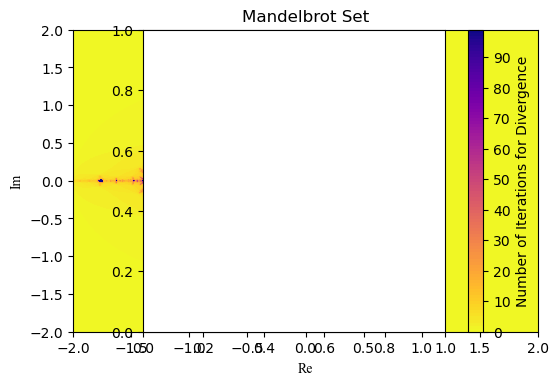
\includegraphics[]{mandelbrot2.png}
    \caption{Mandelbrot set density version}
    \label{fig:1}
    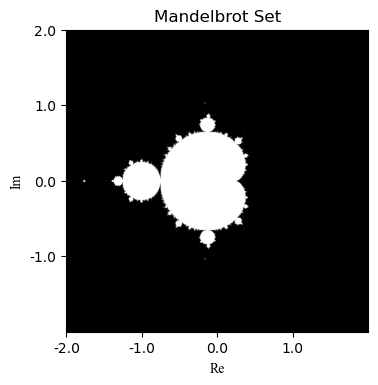
\includegraphics[]{mandlebrot1.png}
    \caption{Mandelbrot set binary version}
    \label{fig:2}
\end{figure}
\newpage
\section{Q2}
\subsection{Method}
For this question a sytems of equations is given by\\
\begin{eqnarray}
\dot X &=& -\sigma(X-Y)\\
\dot Y &=& rX -Y - XZ\\
\dot Z &=& -bZ + XY
\end{eqnarray}
with the initial conditions of $W\equiv(X, Y, Z)$, we will first set up the differential equations for $X,Y,Z$ then followed by the an added time dimension $X,Y,Z,T$ where both will be solved to output following which for the plot we will set up a new function with 6 variable with x, y, z: a point of interest in three dimensional space and $\sigma$, r, b: parameters defining the function. For the plots, the first plot Fig 3 is made by setting the parameters to the number of steps which gives a comprehensive 3D shape and the second plot, Fig 4 is made by setting the number of steps to 5 which give a more simplified version of the plot.
\subsection{Results}
From Figure 4 we can see that at a small step there is no significant interruptions to the plot as seen by the clean plot. However at a greater number of steps we see that spirals develop as the system becomes more chaotic from the propagation of error.
\newpage
\begin{figure}
\subsection{Figures for Q2}
    \centering
    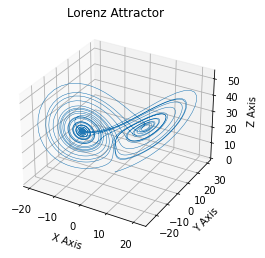
\includegraphics[]{lorenz1.png}
    \caption{Lorenz plot with high number of steps}
    \label{fig:1}
    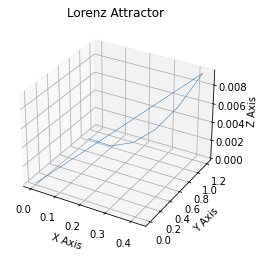
\includegraphics[]{lorenz2.png}
    \caption{Lorenz plot with low number of steps}
    \label{fig:2}
\end{figure}
\newpage
\end{document}
